%!TEX root = ../thesis.tex
% ******************************* Thesis Appendix A ****************************
\chapter{LAG SIM Software Implementations} 

% **************************** Define Graphics Path **************************
\ifpdf
    \graphicspath{{Appendix1/Figs/Raster/}{Appendix1/Figs/PDF/}{Appendix1/Figs/}}
\else
    \graphicspath{{Appendix1/Figs/Vector/}{Appendix1/Figs/}}
\fi

\section{LabVIEW control software} \label{appx:labview-lagsim}
The LAG SIM control software is written in LabVIEW, a graphical programming language which links variables through block diagrams rather than textual functions. 
This makes running tasks simultaneously easier in LabVIEW than other languages, making it ideally suited for instrument control where some events must happen in parallel, and others in a strict order.
A further advantage of LabVIEW is that the user interface is built simultaneously with the program control logic, making it suitable for building applications designed to be run by non-expert end users. 

The user-facing controls of the LAG SIM software are detailed in Section~\ref{sec:labview}. 
This section of the appendix includes some of the block diagram logic that powers the microscope control software, equivalent to presenting source code for other programming languages. 

LabVIEW supports abstraction with inputs and outputs, like functions in other languages, so repeatable pieces of logic can be wrapped up in their own subVI blocks. 
The LAG SIM software is made up of 55 such files, and presenting them all here would be impractical; however, the entire project is available to download from \url{https://github.com/laseranalyticsgroup/sim-labview-control}. 
Here I will present the implementation of LAG SIM's experiment logging feature, since it is a reusable component that could be useful in many other LabVIEW control programs. 

\begin{sidewaysfigure}[p]
\centering
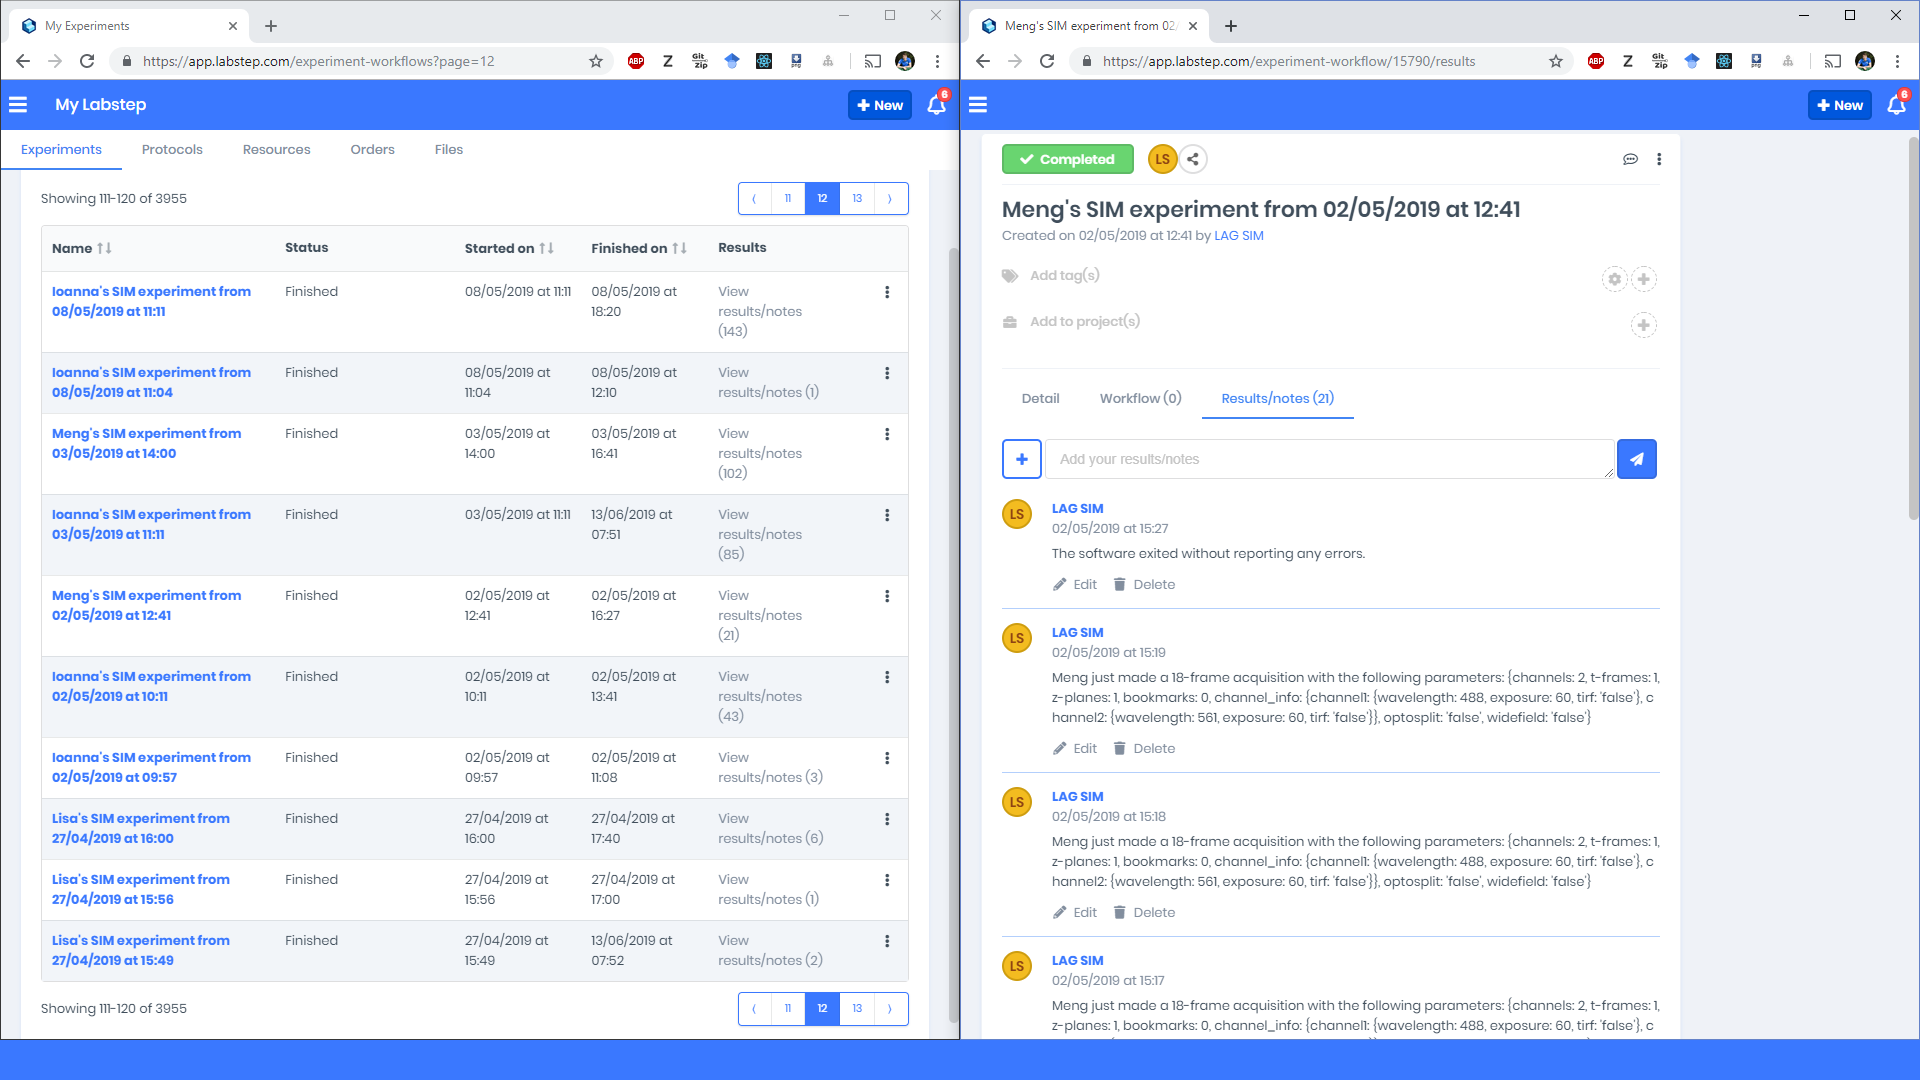
\includegraphics[width=\textwidth]{labstep-timeline}
\caption[Logging user activity with Labstep allows any problems to be identified and fixed quickly]{User activity is automatically logged to an online logbook hosted on Labstep to identify and fix any problems quickly. The left-hand screenshot shows which users have used the LAG SIM between 27-04-2019 and 08-05-2019; opening one of these experiments (right) shows each of the acquisitions they made with the instrument parameters recorded in JSON format.}
\label{fig:labstepTimeline}
\end{sidewaysfigure}

Labstep is an online laboratory management system, designed to make research work compliant, collaborative, and audited. 
Experiments can be logged in an electronic laboratory notebook and, because they are stored online, can be accessed from anywhere with an internet connection.
An example of the Labstep timeline, along with details of an experiment, is shown in Figure~\ref{fig:labstepTimeline}. 
Of particular interest to me was access to the system through an API, allowing requests to be made from any programming language that supports HTTP. 

LabVIEW has built-in functions for making HTTP requests to a remote server. 
To interact with the Labstep API, the functions GET, POST, and PUT are required, each of which has their own block in LabVIEW. 
A full list of API endpoints and the HTTP requests that they respond to can be found at Labstep's website, \url{https://github.com/Labstep/labstep-api-examples}. 

For LAG-SIM, the required functionality was: record which user has started an experiment; post a comment to the experiment timeline every time they capture an image, which records the microscope settings for that acquisition; log any software errors that occurred, which could happen if a piece of hardware is switched off for example; and finally, end the experiment when the user closes the software. 

The block-diagram logic for starting an experiment is shown in Figure~\ref{fig:labstep-implementation}a. 
First, an HTTP request handler is set up, and the API key is added as a header. 
In parallel to this, a JSON string is created which will become the body of the HTTP request, containing a title (`name') for the experiment, and a description of the experiment which contains the time and date formatted as a string. 
The body is POSTed to the appropriate endpoint, \url{https://api.labstep.com/api/generic/experiment-workflow}. 
Finally, the response of the request is parsed to extract the \texttt{Thread ID} and \texttt{Experiment ID}, variables which will be required to add comments to the experiment and to finish the experiment respectively. 
If the subVI cannot extract these IDs, it generates an error; this could occur if, for example, the API key is incorrect or there is no internet connection. 

\begin{figure}[p]
\centering
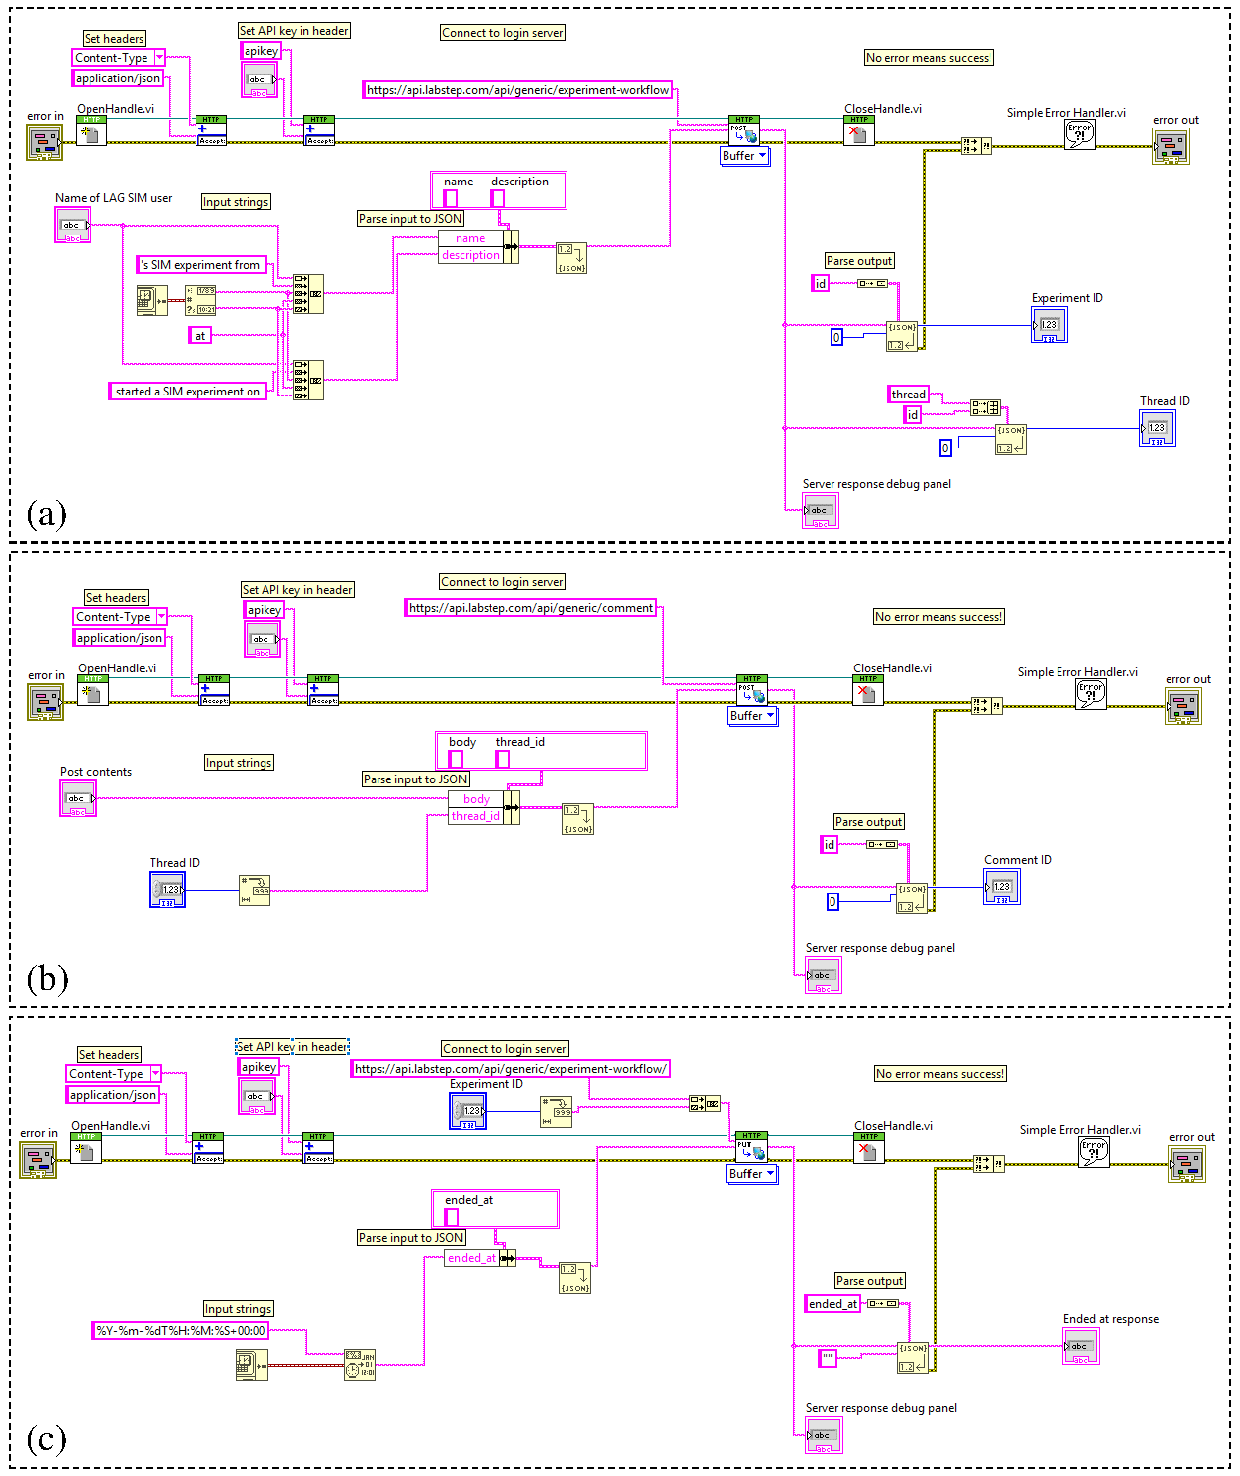
\includegraphics[width=1.0\textwidth]{labstep-implementation}
\caption[SubVIs for uploading experiment information to Labstep]{(a) shows the block diagram logic for creating a new experiment on Labstep with an HTTP request. (b) shows the subVI for adding a comment to the experiment, which can be used to log information about each acquisition. (c) shows the logic for closing the Labstep experiment, which is executed when the LAG SIM control software is closed. }
\label{fig:labstep-implementation}
\end{figure}

The subVI for starting an experiment is shown as part of a larger block diagram in Figure~\ref{fig:labstep-implementation-top}a, where the logic has been abstracted into a block with 2 inputs and 2 outputs. 
The API key is stored in the program, and the user's name is collected from the user when they open the software; the output wires \texttt{Experiment ID} and \texttt{Thread ID} continue into the program to be used again later. 

\begin{figure}[tbp]
\centering
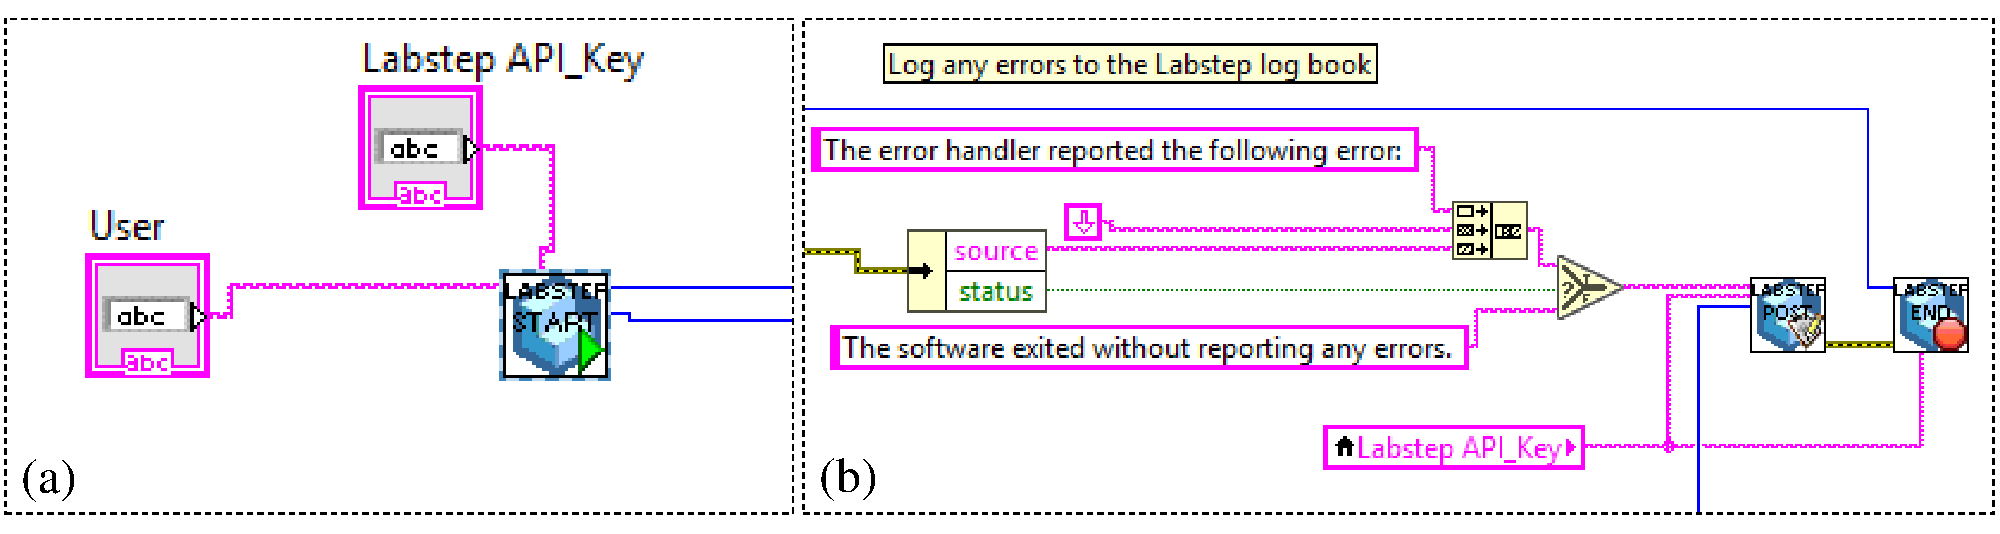
\includegraphics[width=1.0\textwidth]{labstep-implementation-top}
\caption[Top-level LabVIEW functions for uploading to Labstep]{(a) shows the block diagram from Figure~\ref{fig:labstep-implementation}a abstracted to a single block with 2 inputs and 2 outputs. (b) shows the logic that runs when the user exits the LAG SIM control software: any errors are logged to the Labstep timeline for the experiment, using the logic of Figure~\ref{fig:labstep-implementation}b, and finally the experiment is ended with the logic of Figure~\ref{fig:labstep-implementation}c. } 
\label{fig:labstep-implementation-top}
\end{figure}

Figure~\ref{fig:labstep-implementation}b shows the subVI for posting a comment to an experiment.
The inputs are a \texttt{Thread ID}, from the initialisation subVI, and a string, which is any collection of words or characters.
Every time an acquisition is made, this subVI is called with an input string which describes the microscope settings for that particular acquisition. 
This is set up as a JSON string, as shown in Figure~\ref{fig:labstepTimeline}, which leaves potential for further processing on the metadata at a later time. 

When the user has finished their session and closes the software, the snippet shown in Figure~\ref{fig:labstep-implementation-top}b is executed. 
If an error occured during the software execution, this is logged just before the block to end the experiment is executed using the comment-positing subVI detailed in Figure~\ref{fig:labstep-implementation}b. 
Finally, the `END' subVI is called to close the experiment on Labstep; the contents of this block are shown in Figure~\ref{fig:labstep-implementation}c. 

The logging software described in this sectioning is available on the LabVIEW community file exchange, at \url{https://forums.ni.com/t5/Example-Program-Drafts/Logging-with-Labstep/ta-p/3822118}. 
The blocks can be reused in any other LabVIEW program, providing the computer is connected to the internet. 
The full LAG SIM control program, which includes the Labstep integration, is available on Github at \url{https://github.com/laseranalyticsgroup/sim-labview-control}. 

\section{SROS-SIM reconstruction on GPU} \label{appx:gpu-srossim}
When I arrived in the Laser Analytics Group, SIM data was reconstructed using either Lin Shao's algorithm written in CUDA, as described in Section~\ref{sec:shao-recon}, or, when super-resolution with optical sectioning was required, a MATLAB script called SROS-SIM written by Florian Str{\"o}hl was used. 

The main disadvantage of SROS-SIM was its speed. 
A single 1024$\times$1024 frame of SIM data took \SI{22.7}{\second} to reconstruct on the CPU, assuming that illumination parameters such as spatial frequency and phase shift had been calculated beforehand. 
Furthermore, calculating the illumination parameters took \SI{105.2}{\second} although these could be computed once per data set and reused for the set. 

These speeds were impractically slow for high-throughput experiments, where hundreds or, for timelapse data, thousands of SIM frames require reconstruction. 
Furthermore, during an experiment it is often useful to view reconstructed data to ensure imaging conditions are optimal; waiting over two minutes to see a single reconstructed frame is not practical when live cells are surviving in unfavourable conditions on the microscope. 
There was a clear need to increase the speed of the program.

One reason for the particularly slow parameter estimation was an autocorrelation operation, implemented as a convolution.
A direct convolution operation has an algorithmic complexity of $O(n^2)$, where $n$ is the number of elements in the array to be convolved. 
Since the images to be convolved are large 2D arrays, convolution is a particularly expensive operation which becomes exponentially slower the larger the image size. 

\begin{table}[b]
\caption[SROS-SIM reconstruction is 32X faster on the GPU than the CPU]{\label{tab:reconPerformance}The table shows the performance increase by switching from CPU to GPU computation, as well as other optimisations. This test was performed on a consumer desktop computer, with the following specification: 2-core i3-2120\,@\SI{3.30}{\giga\hertz}, \SI{8}{\giga\byte} RAM, NVIDIA GeForce GTX 750 Ti with \SI{2}{\giga\byte} graphics RAM.}
\centering
\begin{tabular}{|l|c|c|}
\hline
\textbf{Condition} & \textbf{Parameter calculation (s)} & \textbf{SIM reconstruction (s)} \\ \hline
CPU & 105.2 & 22.7 \\
CPU with FFT-convolution & 46.7 & 22.7 \\
GPU & 25.5 & 1.3 \\
GPU at single precision & 13.0 & 0.7 \\
\hline

\end{tabular}
\end{table}

A mathematically equivalent operation is shown by Equation~\ref{eq:fourier-correlation}, where $A$ and $B$ are example arrays and $\mathcal{F}^{-1}$ is the inverse Fourier transform. 
This requires Fourier transforming the arrays and a point-wise multiplication of the resulting Fourier-space arrays.
However, several Fast Fourier Transform (FFT) algorithms have been invented which recursively reduce the Fourier transform into smaller arrays, ultimately Fourier transforming with a complexity of $O(n\log n)$, which is faster than $O(n^2)$. 
Implementing the auto-correlation as a Fourier transform gave a 2.25$\times$ improvement in parameter calculation time, shown in Table~\ref{tab:reconPerformance}. 

\begin{equation} \label{eq:fourier-correlation}
A \otimes B \equiv \mathcal{F}^{-1}\left\lbrace\hat{A}\hat{B}\right\rbrace
\end{equation}

The recursive reduction property of FFT algorithms lend themselves well to calculation on a GPU, as each reduced array can be operated on independently of the other arrays. 
GPU architectures, which are designed to run many simple calculations in parallel, are well optimised for this type of problem. 
By moving the arrays onto the graphics memory and computing the FFT on the GPU a further 1.8$\times$ speed improvement was obtained compared to computing the FFT on the CPU. 

More remarkable was the reduction in time required to compute a frame of SIM reconstruction, which also requires many Fourier transforms and simple, pixel-wise calculations which can be computed in parallel. 
By computing the reconstruction on the GPU, a speed increase of 17$\times$ was achieved, as shown in Table~\ref{tab:reconPerformance}. 

A final performance optimisation was realised by reducing the precision to which pixel values were calculated. 
In the original SROS-SIM program, values were calculated to double-precision floating-point format, requiring 64 bits per pixel.
While it is good practice to perform calculations to more precision than required to avoid computational rounding errors, the sCMOS camera only records images to 10-bit precision, so 64 bits is unnecessarily excessive.
Furthermore, graphics cards are usually optimised for single-precision calculations - that is, 32 bits per pixel. 
When arrays were stored and calculated in the single-precision floating point format, Table~\ref{tab:reconPerformance} shows that speed of calculation was almost doubled compared to computation at double precision. 

Overall, an 8$\times$ improvement in speed was achieved for parameter estimation, and a 32$\times$ improvement for per-frame reconstruction time, reducing the time to reconstruct a SIM frame to \SI{0.7}{\second}. 
These improvements made it possible to reconstruct data during acquisition, to see results almost immediately without endangering the longevity of live-cell experiments. 

MALTAB arrays are moved from CPU memory to GPU memory with the \texttt{gpuArray()} function. 
After an array has become a gpuArray, any computations involving the array will be performed by the GPU. 
For computations which can be highly parallelised, for example fast Fourier transforms, this can lead to significant reductions in processing time. 
Once the GPU computations are complete, the array can be moved back to CPU memory with the \texttt{gather()} command, for performing CPU operations such as saving to disk. 

To ensure backwards compatibility on machines without GPUs, the revised code checks if the machine has a GPU and sets a boolean flag \texttt{gpuPresent}, as shown in Snippet~\ref{snip:gpu-check}. 
If this flag is set, the array is sent to GPU with \texttt{gpuArray()}; else, it will be left as a MATLAB matrix which will be computed on the CPU. 

\begin{lstfloat}
\begin{lstlisting}[language=matlab,caption={A check must be performed at the start of the top-level MATLAB program to detect if a suitable graphics card is installed for GPU computation},label={snip:gpu-check},frame=single]
gpuPresent = false; 
if (gpuDeviceCount > 0) 
    try
        g = gpuDevice();
        fprintf(['GPU device detected... \n' ...
            '                 Name: ' g.Name ' \n', ...
            '    ComputeCapability: ' g.ComputeCapability ' \n']);
        % Tested for 3.0 and better
        if(g.ComputeCapability > 3.0)
            disp('Device supported, executing on GPU... '); 
            gpuPresent = true; 
        else
            disp(['GPU functionality requires ComputeCapability' ...
                ' of 3.0 or higher. Executing on CPU... ']); 
        end
    catch
        disp('GPU device not compatible. Executing on CPU..');
    end
end
\end{lstlisting}
\end{lstfloat}


To save writing a conditional check around every single array, a simple wrapper function shown in Snippet~\ref{snip:gpu-array} called \texttt{gpuThis()} was created, which takes as input arguments the array to potentially send to the GPU, and the \texttt{gpuPresent} variable calculated in Snippet~\ref{snip:gpu-check}.

\begin{lstfloat}
\begin{lstlisting}[language=matlab,caption={A simple helper function, \texttt{gpuThis()}, sends an array to graphics memory if a GPU is available, but leaves the array in CPU memory if not},label={snip:gpu-array},frame=single]
function output = gpuThis(input, GPU_present);

if GPU_present
    output = gpuArray(single(input));
else
    output = single(input);
end

end
\end{lstlisting}
\end{lstfloat}

To make the program GPU-optimsed, we now simply put \texttt{gpuThis()} around each array that would benefit from GPU computation during its allocation. 
Snippet~\ref{snip:gpuThis-use} shows a small extract from the original SROS-SIM code in lines 1-6, responsible for loading the OTF for each channel into a 3-dimensional array. 
The changes highlighted in lines 8-13 show that only 2 lines need modification for GPU optimisation. 

\setlength\fboxsep{0pt}
\begin{lstfloat}
\begin{lstlisting}[language=matlab,caption={The function \texttt{gpuThis()} should be wrapped around new arrays when they are preallocated},label={snip:gpuThis-use},frame=single,escapechar=$]
$\colorbox{red!20}{otf = zeros(HEIGHT,WIDTH,SETUP.colours);}$
for c = 1:SETUP.colours
  $\colorbox{red!20}{otf(:,:,c) = }$$\colorbox{red!50}{double(}$$\colorbox{red!20}{imread([DATA.OTF\_path\{c\}, DATA.OTF\_name\{c\}, DATA.OTF\_suffix\{c\}]));}$
  % Normalise
  otf(:,:,c) = otf/max(max(otf(:,:,c)));
end

$\colorbox{green!20}{otf = }$$\colorbox{green!50}{gpuThis(}$$\colorbox{green!20}{zeros(HEIGHT,WIDTH,SETUP.colours)}$$\colorbox{green!50}{, gpuPresent)}$$\colorbox{green!20}{;}$
for c = 1:SETUP.colours
  $\colorbox{green!20}{otf(:,:,c) = }$$\colorbox{green!50}{gpuThis(}$$\colorbox{green!20}{imread([DATA.OTF\_path\{c\}, DATA.OTF\_name\{c\}, DATA.OTF\_suffix\{c\}])}$$\colorbox{green!50}{, gpuPresent}$$\colorbox{green!20}{);}$
  % Normalise
  otf(:,:,c) = otf/max(max(otf(:,:,c)));
end
\end{lstlisting}
\end{lstfloat}

The small wrapper function \texttt{gpuThis} could be used in any other MATLAB code to investigate whether it benefits from GPU computation. 
The biggest speed increases will be achieved when large matrices require Fourier transforming, or other operations which can be computed in parallel. 

The full SROS-SIM software, with the new GPU optimisations, is hosted at \url{https://github.com/laseranalyticsgroup/jRL-SIM}. Access to the repository is available upon request. 


\section{ImageJ/Fiji plugin} \label{appx:fiji-lagsim}
The LAG SIM plugin for ImageJ makes reconstructing artefact-free SIM data straightforward for users who are not experts in SIM reconstruction algorithms. 
The user interface is detailed in Section~\ref{sec:lagsimFiji}. 
This appendix contains extracts from the source code explaining the technical implementation of the plugin. 

The plugin is implemented in Beanshell, a scripting language which closely resembles Java but allows execution without the need for compilation. 
The plugin is built upon functions provided by the fairSIM project from Marcel M{\"u}ller~\cite{muller2016open} and the Squirrel project from Si{\^a}n Culley~\cite{culley2018quantitative}. 
These projects include efficient and accurate algorithms, but have generic user interfaces which requires unnecessarily repetitive clicking by LAG SIM users. 
The LAG SIM plugin combines the two projects into one user interface, and automatically inputs the appropriate parameters for our instrument. 

The plugin includes a function for batch SIM reconstruction, and a parameter finder for choosing optimal reconstruction parameters. 
Extracts from the parameter finder source code are presented in Snippet~\ref{snip:lagsim-fiji}; the full source code is available from the ImageJ update site for LAG SIM at \url{https://sites.imagej.net/LagSIM}. 

Lines 1-6 begin with \texttt{//@}, which is an ImageJ-specific syntax for automatically creating a dialog box with these inputs when the function is executed. 
Furthermore, specifying the input parameters in this syntax allows the function to be called with custom parameters from an ImageJ macro, which could be useful for future users who want to implement the parameter finder as part of a larger program. 

Lines 8-13 show a sample of the modules which need to be imported for the Beanshell script to function properly. 
Most modules are included with a standard ImageJ installation; however, fairSIM and NanoJ-Squirrel are notable dependencies which must be installed separately. 
Both projects are distributed as ImageJ update sites, available in the ImageJ update menu. 

The first task for the parameter finder is to set the instrument parameters based on the lens and wavelength used on LAG SIM, shown in lines 22-49. 
In the native fairSIM plugin, these would need to be entered every time a SIM reconstruction is required; abstracting the values into the LAG SIM plugin saves users time and reduces errors, since users do not have to remember lots of arbitrary numbers. 
Furthermore, in batch mode the LAG SIM plugin is able to extract wavelength and lens information directly from the filename, removing the need for any user input. 

Line 59 calls the fairSIM function \texttt{estimateParameters}, which extracts the spatial frequency and phase shift of the illumination pattern to sub-pixel accuracy. 
Lines 62-78 check the modulation depth of the illumination pattern, and warns the user if it looks low.
This may mean there is too much out-of-focus light in the image for a reliable reconstruction, or the lens and wavelength combination may be incorrect. 

Lines 90-101 set up and execute the fairSIM reconstruction algorithm for the test image.
This runs in a \texttt{while} loop, so that the user can continue to test parameters until the press the \texttt{Finish} button. 
Each additional test image is added to \texttt{outputStack}, so that the user can compare visually how different parameters affect the reconstruction. 

If the \texttt{Calculate Squirrel metrics} checkbox is ticked, lines 105-107 generate a widefield image to use as the Squirrel reference image. 
Line 109 then calls Squirrels \texttt{"Calculate Error-Map, RSE and RSP"} function as an ImageJ macro, automatically entering the appropriate inputs. 
The RSP and RSE values are extracted from Squirrel's results window in lines 112-116, and added to LAG SIM's results window in lines 118-123, along with the test number and reconstruction parameters used. 

Finally, in lines 129-133 the final SIM parameters tested are saved to the ImageJ preferences file. 
If the parameter tester or batch reconstruction plugins are run without inputs, these values will be loaded in as the default parameters, so that the user does not have to write them down and re-enter them. 

\clearpage
\begin{lstlisting}[language=java,caption={Extracts from the Beanshell script used for the LAG SIM parameter tester},label={snip:lagsim-fiji},frame=single]
//@String(label="Filter type", choices={"Wiener out", "RL out", "RL in, Wiener out", "RL in, RL out"}) filter
//@Double(label="Wiener Parameter", value=0.05) wienerParameter
//@Double(label="Apodisation cutoff", value=1.9) apoCutoff
//@Double(label="Apodisation strength", value=0.8) apoBend
//@Integer(label="Richardson-Lucy steps", value=5) rlSteps
/* etc. */

import ij.IJ;
import ij.ImagePlus;
import ij.ImageStack;
import org.fairsim.sim_algorithm.SimAlgorithm;
import nanoj.squirrel.java.gui.ErrorMap_;
/* etc. */

// Check active image only has 9 frames: we want this to be quick! 
ImagePlus iPl = ij.WindowManager.getCurrentImage();
if (iPl.getStackSize() != 9){
	MessageDialog errorDlg = new MessageDialog(null, "Raw data stack size error!", "Please use a single-slice, single-channel image for parameter finding.");
	return;
}

// Find illumination parameters with fairSIM
int nrAng   = 3;		// #angles
int nrPha   = 3;		// #phases

switch(lens){
	case "60X Water":
		otfNA = 1.2;
		pxlSize = 0.0833;
	break;
	case "100X Oil":
		oftNA = 1.49;
		pxlSize = 0.05;
	break;
}

switch(wavelength){
	case "488": // 488nm
		emWavelen = 525; 
		px1 = -0.056;
		py1 = -114.567;
		px2 = 99.744;
		py2 = 57.189;
		px3 = -99.811;
		py3 = 57.389;
		break;
	case "561": // 561nm
		/* etc. */
}

OtfProvider otf   = OtfProvider.fromEstimate( otfNA, emWavelen, otfCorr );
SimParam simParam = SimParam.create( nrBands, nrAng, nrPha, imgSize, pxlSize, otf );

// Set initial guesses for parameters
simParam.dir(0).setPxPy(px1, py1);
simParam.dir(1).setPxPy(px2, py2);
simParam.dir(2).setPxPy(px3, py3);

SimAlgorithm.estimateParameters( simParam, rawImages, fitBand, -1, idf, visualFeedback, null);

// Check modulation depth 
double mod0 = simParam.dir(0).getRawModulations()[1];
double mod1 = simParam.dir(1).getRawModulations()[1];
double mod2 = simParam.dir(2).getRawModulations()[1];
					
if (mod0 < 0.5 || mod1 < 0.5 || mod2 < 0.5){
	modStr = "Modulation depth looks quite low. Continue? \n";
	modStr += "\n Modulation dir1: " + String.format("%.2f", mod0);
	modStr += "\n Modulation dir2: " + String.format("%.2f", mod1);
	modStr += "\n Modulation dir3: " + String.format("%.2f", mod2);
						
	GenericDialog modDlg = new GenericDialog("Modulation information");
	modDlg.addMessage(modStr);
	modDlg.showDialog();
						
	if(modDlg.wasCanceled())
		return;
}

// Set up test reconstructions, and loop until user selects finish from the dialog
ImageStack outputStack = new ImageStack(2*imgSize, 2*imgSize);
boolean finished = false;

while (!finished){
	if(simDlg.wasCanceled()){
		finished = true;
		break;
	} else {
		// Set up reconstruction
		simParam.setWienerFilter( wienerParameter );
		simParam.setRLiterations( (int)rlSteps );
		simParam.setFilterStyle( filterStyle );
		/* etc. */
		
		// Run reconstruction! 
		Vec2d.Real result = SimAlgorithm.runReconstruction( simParam, rawImages, idf, visualFeedback, otfBeforeShift, clipscale, null );
		
		// Add reconstruction to test stack
		String testParams = filter + ", w: " + wienerParameter + ", RL: " + (int)rlSteps + ", apoC: " + apoCutoff + ", apoS: " + apoBend + ", at?: " + (otfAttenuation ? "true" : "false") + ", attFW: " + attenFWHM +  ", atS: " + attenStrength; 
		FloatProcessor fp = new FloatProcessor(2*imgSize, 2*imgSize, res);
		outputStack.addSlice(testParams, fp);
		
		if (metrics){
			// Create widefield projection as Squirrel reference image
			ZProjector projector = new ZProjector().setImage(iPl);
			ImagePlus widepl = projector.getProjection();
			widepl.setTitle("squirrel-wf");
		
			IJ.run("Calculate Error-Map, RSE and RSP", "reference=[squirrel-wf] super-resolution=[squirrel-sr] rsf=[-- RSF unknown, estimate via optimisation --] max.=5 crop enable maximum=0 show show_rsf-convolved");
		
			// Extract metrics from Squirrel table, and add to LAG SIM test table
			Window rw = WindowManager.getWindow("RSP and RSE values");
			ResultsTable rt = rw.getResultsTable();
			double rsp = rt.getValue("RSP (Resolution Scaled Pearson-Correlation)", 0);
			double rse = rt.getValue("RSE (Resolution Scaled Error)", 0);
			rw.close();

			testResults.incrementCounter();
			testResults.addValue("Test #", testNumber);
			testResults.addValue("Squirrel RSP", rsp);
			testResults.addValue("Squirrel RSE", rse);
			testResults.addValue("Parameters", testParams);
			testResults.show("Test results");		
		}
	}
}

// Save parameters to ImageJ preferences
Prefs.set("lagsim.filter", filter);
Prefs.set("lagsim.wienerParameter", String.valueOf(wienerParameter));
Prefs.set("lagsim.rlSteps",  String.valueOf(rlSteps));
Prefs.set("lagsim.apoCutoff",  String.valueOf(apoCutoff));
/* etc. */

\end{lstlisting}